\documentclass[final]{beamer}
\usepackage[orientation=portrait,size=a1,scale=1.18]{beamerposter}
\geometry{hmargin=1.5cm,vmargin=0cm}
\usepackage[utf8]{inputenc}
\linespread{1.04}

% Custom theme
\usetheme{sharelatex}
\definecolor{primary}{RGB}{160,32,60}

% Packages
\usepackage{booktabs}
\usepackage{amsmath,amssymb}
\usepackage{graphicx}
\usepackage{tikz}
\usetikzlibrary{shapes, arrows.meta, positioning, calc, fit}
\usepackage{multicol}
\usepackage{url}
\usepackage{xcolor}
\definecolor{progreen}{RGB}{34,139,34}
\definecolor{conred}{RGB}{200,30,30}
\newcommand{\pro}{\textcolor{progreen}{\textbf{+}}}
\newcommand{\con}{\textcolor{conred}{\textbf{--}}}

% Compact list spacing
\usepackage{enumitem}
\setlist[itemize]{leftmargin=1.5em, itemsep=0.1em, parsep=0pt, topsep=0.1em}

\setlength{\columnsep}{2cm}
\usepackage[backend=bibtex, style=numeric, sorting=none, maxnames=2, minnames=1]{biblatex}
\AtBeginBibliography{
  \fontsize{16.15}{7}\selectfont
  \setlength{\itemsep}{0pt}
  \setlength{\parskip}{0pt}
}
\addbibresource{bibliography.bib}

% Title, authors, date
\title[Reinforcement Learning -- CentraleSup\'elec]{Comparative Study of Deep Reinforcement Learning Methods on the Game of Snake}
\author{Fotios Kapotos, Adonis Jamal, Jean-Vincent Martini}
\institute[CentraleSup\'elec]{CentraleSup\'elec}
\date{\today}

% ==============================================================================
\begin{document}
\begin{frame}[t]
\vskip0.1cm
\begin{multicols}{2}

%% ---- COLUMN 1 ----

%% INTRODUCTION & PROBLEM DEFINITION
\begin{block}{1. Introduction \& Problem Definition}

\textbf{Context.}
Reinforcement Learning (RL) has achieved remarkable success in sequential decision-making, from Atari games~\cite{mnih2015human} to Go~\cite{silver2016mastering} and robotics~\cite{singh2022reinforcement}. The \textbf{Snake game} offers a compelling yet underexplored benchmark: its rules are simple, but the strategic requirements are complex.

\smallskip
\textbf{Challenges.}
\begin{itemize} 
  \item The agent must balance \textbf{immediate rewards} (food collection) with \textbf{long-term survival} (avoiding self-collision).
  \item \textbf{As the snake grows, the state space complexity increases} and navigation becomes progressively constrained.
  \item Greedy strategies inevitably fail: \textbf{the agent must plan long trajectories} to avoid trapping itself.
  \item These dynamics mirror real-world problems where available actions diminish over time.
\end{itemize}

\smallskip
\textbf{State of the Art.} 
Focus on Deep Q-Networks (DQN) with convolutional neural networks~\cite{wei2018autonomous}, differing in their state representations (raw pixels versus sensor-based inputs~\cite{sebastianelli2021deep}, reward shaping strategies~\cite{almalki2019exploration}, and memory efficiency~\cite{tushar2022memory}) with some works also comparing alternative algorithms such as SARSA and PPO~\cite{bonnici2021exploring}.

\bigskip

\begin{figure}
\centering
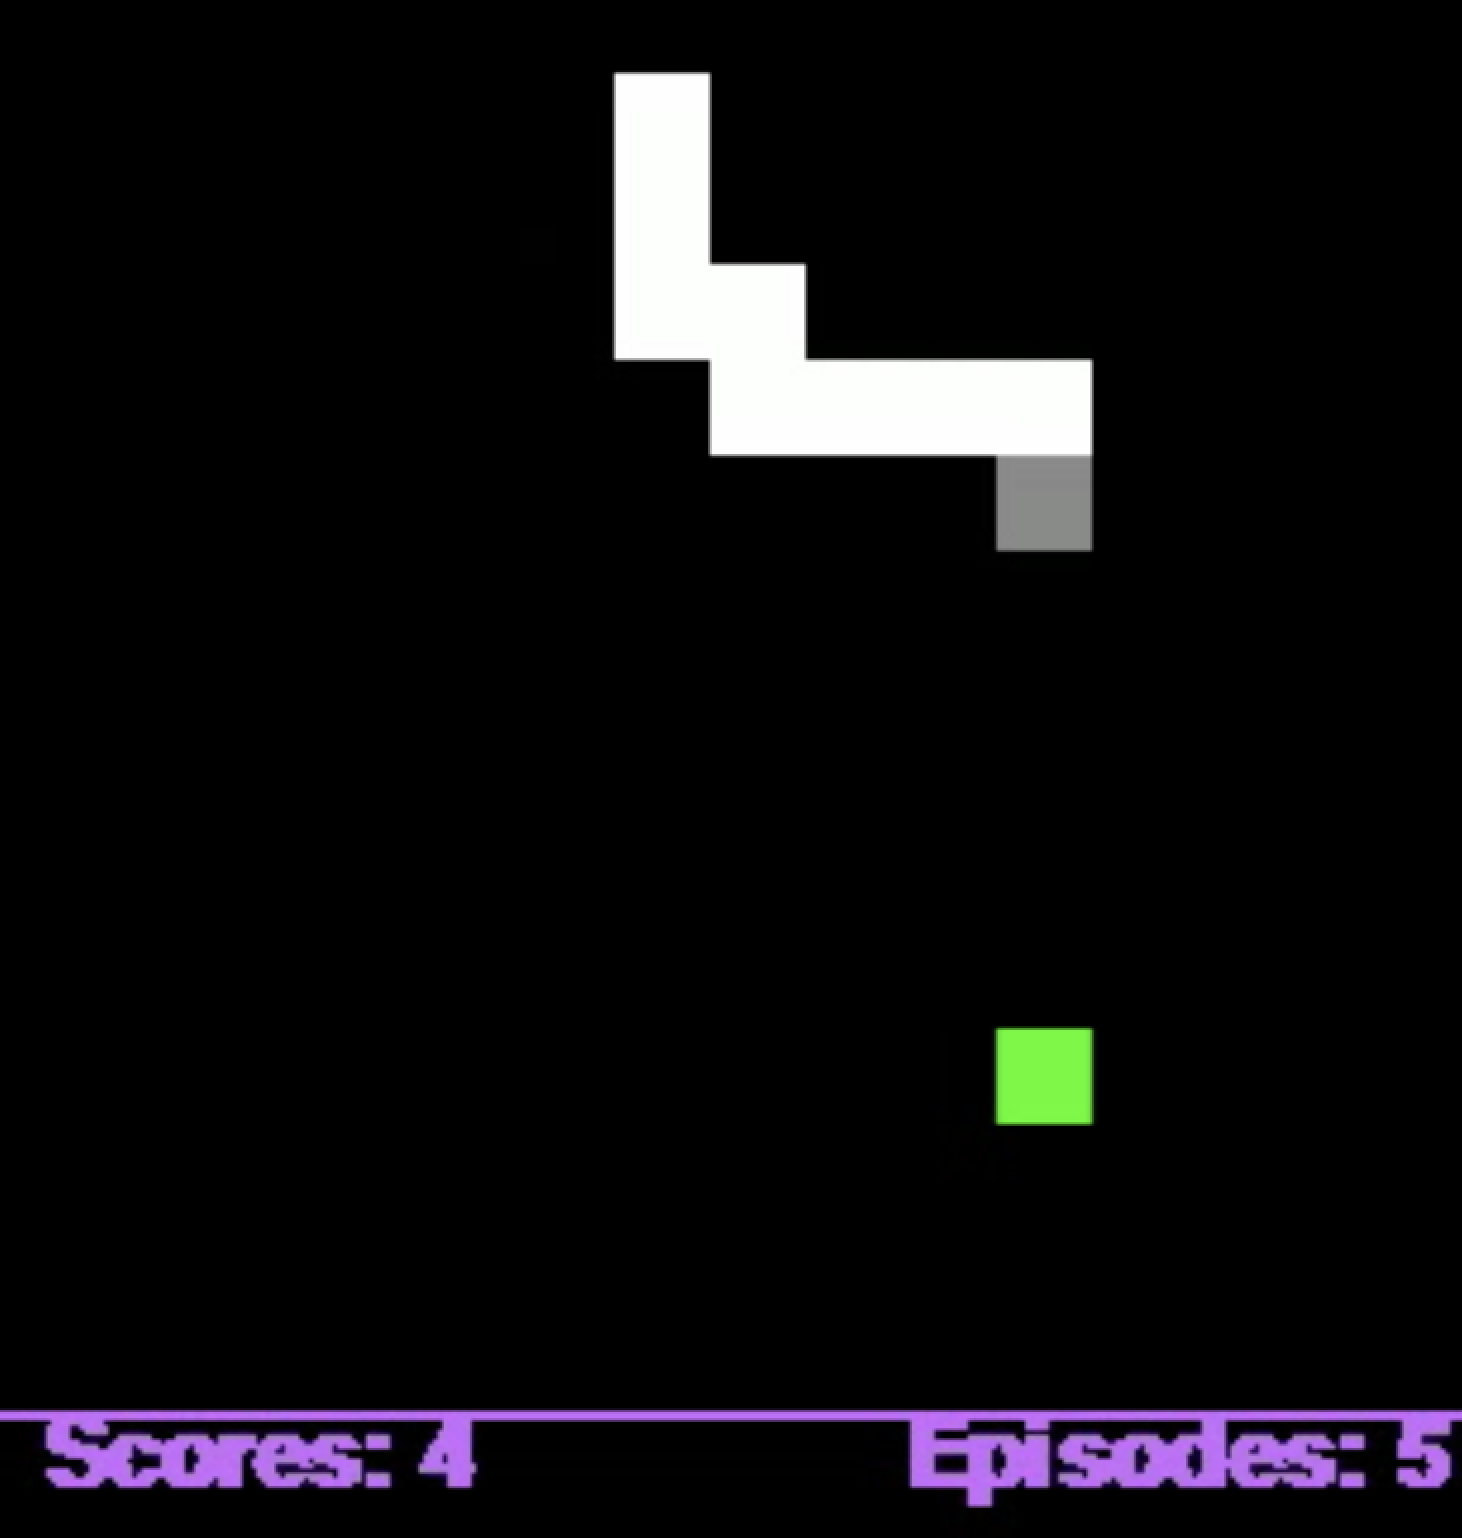
\includegraphics[width=0.4\linewidth]{img/screen_snake.png}
\caption{Snapshot of the Snake environment. The agent (white with grey head) must navigate to collect food (green) while avoiding collisions with itself and walls.}

\end{figure}

\end{block}

%% OBJECTIVES & CONTRIBUTIONS
\begin{alertblock}{2. Objective \& Main Contributions}

\textbf{Objective.} Conduct a systematic empirical comparison of modern deep RL algorithms on the Snake environment, \textbf{investigating how algorithmic choices, reward shaping strategies, and state representations affect learning efficiency and final performance}.

\smallskip
\textbf{Main Contributions.}
\begin{itemize}
  \item A \textbf{comparative analysis} of value-based (DQN, Double DQN) and policy-based (A2C, PPO) methods on a growing-horizon task.
  \item An in-depth study of \textbf{reward shaping} (sparse vs.\ dense) in an environment with naturally delayed consequences.
  \item A comparison of \textbf{multiple state representations}: full grid, egocentric view, and hand-crafted features.
  \item Two neural network policies: a standard \textbf{MLP} and a custom \textbf{CNN} preserving spatial structure.
\end{itemize}

\end{alertblock}

%% METHODOLOGY -- Part 1
\begin{block}{3. Methodology}

\textbf{3.1\quad Algorithms.}

\smallskip
We implement four deep RL agents sharing comparable architectures for fair comparison:

\smallskip
\textbf{DQN}~\cite{mnih2015human} -- \textit{Value-based, off-policy.} Learns an action-value function $Q(s,a)$ via experience replay and a target network.
\begin{itemize}
  \item[\pro] Sample efficient through replay buffer, stable with target network.
  \item[\con] Prone to overestimation of Q-values, discrete actions only.
\end{itemize}

\smallskip
\textbf{Double DQN}~\cite{van2016deep} -- \textit{Value-based, off-policy.} Decouples action selection from evaluation: $a^* = \arg\max_a Q_\theta(s',a)$, evaluated as $Q_{\theta^-}(s', a^*)$.
\begin{itemize}
  \item[\pro] Reduces overestimation bias, more accurate value estimates.
  \item[\con] Still limited to discrete actions, moderate additional complexity.
\end{itemize}

\smallskip  
\textbf{A2C}~\cite{mnih2016asynchronous} -- \textit{On-policy, actor-critic.} The actor learns a policy $\pi_\theta(a|s)$ while the critic estimates $V(s)$ to compute an advantage baseline.
\begin{itemize}
  \item[\pro] Reduced variance via baseline, supports continuous actions.
  \item[\con] On-policy: lower sample efficiency, sensitive to hyperparameters.
\end{itemize}
 
\smallskip
\textbf{PPO}~\cite{schulman2017proximal} -- \textit{On-policy, policy gradient.} Clipped surrogate objective: $L^{\text{CLIP}}(\theta) = \mathbb{E}\!\left[\min\!\left(r_t(\theta)\hat{A}_t,\; \text{clip}(r_t(\theta), 1\!\pm\!\epsilon)\hat{A}_t\right)\right]$.
\begin{itemize}
  \item[\pro] Stable updates via trust region, robust across tasks.
  \item[\con] On-policy: requires large batches, computationally heavier per update.
\end{itemize}

\bigskip
\textbf{3.2\quad Neural Network Policies.}

\smallskip
\textbf{MLP Policy.} A fully-connected network that takes a \textbf{flattened state vector} as input. Used with the full grid (768-dim), egocentric (147-dim), and feature vector (10-dim) encodings. Simple and fast to train.

\smallskip
\textbf{CNN Policy.} A custom convolutional feature extractor preserving the \textbf{spatial} $16\!\times\!16\!\times\!3$ grid structure. Two convolutional layers (16 and 32 filters, $3\!\times\!3$ kernels) followed by a 256-unit fully-connected layer. Enables the agent to learn \textbf{spatial patterns} (walls, body segments, food proximity) directly from the grid.
\end{block}

%% ---- COLUMN 2 ----
\columnbreak

%% METHODOLOGY -- Part 2
\begin{block}{}
\textbf{3.3\quad Modular Wrapper.}

\smallskip
We designed a \texttt{ModularSnakeWrapper} built on top of Gymnasium that \textbf{decouples state encoding and reward computation} from the base environment, enabling systematic experimentation.

\smallskip
\textbf{State Encoders} (interchangeable via configuration):
\begin{itemize}
  \item[{\color{green}$\star$}] \textbf{Full Grid}: flattened $16\!\times\!16\!\times\!3$ board $\rightarrow$ 768-dim vector (MLP) or 3D tensor (CNN).
  \item[{\color{red}$\star$}] \textbf{Egocentric}: $7\!\times\!7$ window centered on the head $\rightarrow$ 147-dim vector (MLP) or 3D tensor (CNN).
  \item[{\color{blue}$\star$}] \textbf{Feature Vector}: 10 hand-crafted features (food direction, danger indicators, normalized distances).
\end{itemize}

\smallskip
\textbf{Reward Functions} (interchangeable via configuration):
\begin{itemize}
  \item[{\color{red}$\star$}] \textbf{Sparse}: \textcolor{progreen}{$+1$} for food, \textcolor{conred}{$-1$} for death/timeout. Minimal signal.
  \item[{\color{green}$\star$}] \textbf{Dense}: \textcolor{progreen}{$+10$} for food, \textcolor{conred}{$-10$} for death. Includes Manhattan distance shaping ($\Delta d \cdot \alpha$), loop detection penalty (\textcolor{conred}{$-8$} when a position is visited $\geq 4$ times in a window of 20 steps), and timeout penalty (\textcolor{conred}{$-5$}).
\end{itemize}

\smallskip
The wrapper also tracks episode step counts and maintains previous-step information for reward computation.

\end{block}

%% EXPERIMENTAL SETUP & RESULTS
\begin{block}{4. Experimental Setup \& Results}

\textbf{Setup.}
All agents are trained for \textbf{5{,}000{,}000 timesteps} on a $16\!\times\!16$ grid using the Gymnasium \texttt{Snake-v1} environment with our custom wrapper. Key hyperparameters: TODO.

\smallskip
\textbf{Evaluation Metrics.}
\begin{align*}
  &\text{Average score (food collected)} && \text{Maximum snake length} \\
  &\text{Survival time (steps)} && \text{Cumulative reward}
\end{align*}

\bigskip
\textbf{Results.}

\bigskip
\begin{center}
\textit{[Placeholder: Learning curves -- Average reward vs.\ training steps for all agents]}
\end{center}

\bigskip
\begin{center}
\textit{[Placeholder: Bar plot -- Average food collected per agent and state representation]}
\end{center}

\bigskip
\begin{center}
\textit{[Placeholder: Reward shaping comparison -- Sparse vs.\ dense reward across agents]}
\end{center}

\bigskip

\end{block}

%% CONCLUSIONS
\begin{block}{5. Conclusions}
\begin{itemize}
    \item Dense rewards and CNN policies significantly outperform sparse rewards and MLP baselines on the Snake game. TODO
    \item Our modular wrapper enables systematic ablation of state representations and reward functions, providing a reusable benchmark for grid-based RL.
\end{itemize}
\end{block}

%% REFERENCES
\begin{block}{References}
{\tiny
\printbibliography[heading=none]
}
\end{block}

\end{multicols}
\end{frame}
\end{document}
